\section{Evaluation}
\label{sec:evaluation}

% Results figures, rendered from the persisted artifacts:
% bootstrap_ci.json (suite means and 95% CIs), stability_run1_vs_run2.json (run pairs).
% Layout discipline: the top panel shows point estimates + intervals only
% (no filled bars under the whiskers), the bottom panel's legend lives
% below the axis (never over the bars), and both panels share the same
% value range so the stacked scales read as one.
\begin{figure}[t]
\centering
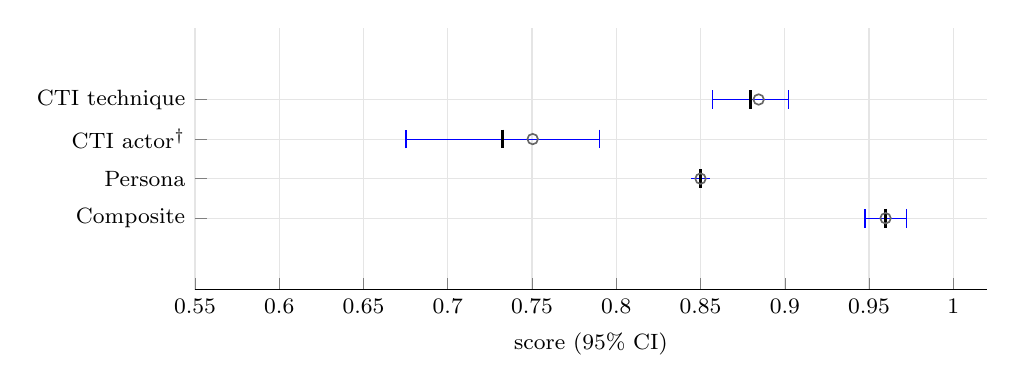
\begin{tikzpicture}
\begin{axis}[
  name=ax1,
  width=0.96\linewidth,
  height=4.9cm,
  xmin=0.55, xmax=1.02,
  y axis line style={draw=none},
  axis x line*=bottom,
  axis y line*=left,
  ytick=data,
  yticklabels={Composite,Persona,CTI actor$^{\dagger}$,CTI technique},
  y dir=reverse,
  xlabel={score (95\% CI)},
  xlabel style={font=\footnotesize},
  tick label style={font=\footnotesize},
  enlarge y limits=0.6,
  grid=major,
  grid style={black!10},
  clip=false
]
% point estimates and bootstrap 95% CIs from bootstrap_ci.json;
% only marks + intervals: no bars beneath the whiskers
\addplot+[only marks, mark=|, mark size=3.4, mark options={thick,black},
  error bars/.cd, x dir=both, x explicit] coordinates {
  (0.9598,3) +- (0.0122,0.0122)
  (0.8500,2) +- (0.0000,0.0000)
  (0.7325,1) +- (0.0573,0.0558)
  (0.8796,0) +- (0.0224,0.0204)
};
% run-2 overlay: open markers (point estimates from stability_run1_vs_run2.json;
% per-suite CIs were not computed for run 2, so none are drawn)
\addplot+[only marks, mark=o, mark size=1.9, mark options={semithick,black!60}] coordinates {
  (0.9598,3)
  (0.8500,2)
  (0.7504,1)
  (0.8845,0)
};
\end{axis}
\end{tikzpicture}

\vspace{2mm}

\begin{tikzpicture}
\begin{axis}[
  name=ax2,
  width=0.96\linewidth,
  height=4.9cm,
  ybar=1.5pt,
  bar width=9pt,
  ymin=0.55, ymax=1.0,
  symbolic x coords={CTI technique,CTI actor,Persona,Composite},
  xtick=data,
  ylabel={mean score},
  ylabel style={font=\footnotesize},
  tick label style={font=\footnotesize},
  ymajorgrids,
  grid style={black!10},
  enlarge x limits=0.25,
  legend style={font=\scriptsize, at={(0.5,-0.16)}, anchor=north, legend columns=2, draw=none, fill=none},
  legend cell align={left},
]
% run 1 vs run 2 from stability_run1_vs_run2.json
\addplot+[black!35, fill=black!35] coordinates {
  (CTI technique,0.9598) (CTI actor,0.8500) (Persona,0.7325) (Composite,0.8796)
};
\addplot+[black!70, fill=black!70, pattern=north east lines] coordinates {
  (CTI technique,0.9598) (CTI actor,0.8500) (Persona,0.7504) (Composite,0.8845)
};
\legend{run 1, run 2}
\end{axis}
\end{tikzpicture}
\caption{Live-campaign results from the persisted artifacts. \emph{Top:}
suite means with bootstrap 95\% confidence intervals; open markers mark
the independent second run's point estimates, and the actor interval is
degenerate ($^{\dagger}$) because the actor rubric assigns the same
score to every row, so uncertainty is carried by the Wilson pass-rate
interval instead (Table~\ref{tab:live}). \emph{Bottom:} two independent
218-query campaigns; the deterministic CTI strata replicate exactly and
only the LLM-judged persona stratum moves, by $+0.018$.}
\label{fig:results}
\end{figure}


The evaluation asks whether each mechanism the design introduces
contributes measurably. We organize it by the four research questions of
\S\ref{sec:intro}: the value of grounding (RQ1), consistency and safety
under adversarial interaction (RQ2), deception quality under an
independent LLM judge panel (RQ3), and the escalation pricing of each
intelligence rung (RQ4), followed by run-to-run stability and threats to
validity. Every quantitative claim in this section is traceable to a
persisted artifact in the released benchmark suite; where an interval is
reported it is a bootstrap 95\% confidence interval computed over paired
rows.

\subsection{Experimental Setup}
\label{sec:setup}

\subsubsection{Testbed}
All experiments run on the production single-host deployment described in
\S\ref{sec:implementation} (2~vCPU, ${\sim}4$~GB RAM). Generative
components use two model families from one free-tier provider: a generator
for deception drafts and a judge model for evaluation, chosen from a
different family than the generator. The provider catalog and quota are
probed by a scheduled watcher; one catalog removal (a third model) and one
quota-exhaustion window occurred during the study, both logged by the
watcher and both handled by the fallback path of \S\ref{sec:fallback}.

\subsubsection{Workloads}
Three query suites exercise the loop end to end:
\emph{CTI-technique} (123 queries asking how specific \attck techniques
are abused, scored on grounded technique coverage),
\emph{CTI-actor} (35 queries on named threat-actor behavior, scored on
attribution quality), and \emph{persona-realism} (60 interactive sessions
driven by scripted attacker personas, scored by an LLM judge on
host-believability rubrics). One scope note: the technique and actor
suites are retrieval question-answering through the loop's CTI path,
not attacker interactions; the attacker-interaction evidence in this
paper is the persona stratum, the C1 re-query battery, and the
ablation/consensus scenarios, and the composite should be read
accordingly. Each suite runs through the full verified
loop with HITL auditing enabled. The scenario sets are fixed and released,
so every run below is a re-run of the same 218 sessions.

\subsubsection{Metrics}
Suite scores are normalized to $[0,1]$ with a per-scenario pass threshold;
composite is the row-weighted mean (technique and actor rows are scaled
to a common range by the released scorer, so the equal-size suite
averaging is well defined). For the ablation we report
paired-difference bootstrap CIs, pairing rows by scenario across arms.
For consistency we report contradiction rate over targeted re-queries.
For deception quality we report a 1--5 rubric consensus over three
evaluator personas, scored on five dimensions: \emph{deception realism}
(would the output pass as the claimed service), \emph{persona
consistency} (does content match the attacker's skill tier), \emph{TTP
accuracy} (are the extracted \attck mappings correct and complete),
\emph{engagement} (does the response invite continued interaction rather
than dead-ending), and \emph{artifact safety} (is served credential
material registered canary bait rather than leakage). Each evaluator
also records a rationale per dimension; these rationales are what
located the harness defect and the fiction contradiction reported below.
All intervals in this section are Wilson 95\% intervals for pass rates
and percentile bootstrap 95\% intervals (10{,}000 resamples, fixed
seed 20260922) for continuous means; the code and seed are
released with the artifacts.

The CTI suites are scored by fixed, released string-matching rubrics,
not by a model. The \emph{technique} rubric scores a response 0--1 by
string evidence: 0.8 if the response contains the expected technique
identifier, $+0.3$ if it contains the parent technique, $+0.1$ for
explicit ATT\&CK framing (capped at 1), and name-variant matching when
the identifier is absent; the \emph{actor} rubric scores 0.5 for the
expected actor name, $+0.3$ for the sector, and $+0.1$ for
campaign-language markers (capped at 1). Two consequences follow, and
we state them rather than let them blur. First, these rubrics measure
the surface delivery of the expected intelligence; they cannot certify
semantic correctness, which is why the TTP-accuracy dimension of the
consensus study and the released transcripts matter. Second, the
rubrics are identical across ablation arms, so the paired differential
measures what grounding changes about delivery, not extraction
plumbing; the raw 35-vs-0 technique count below is analyzed
correspondingly as a dependence result. Third --- a defect not designed
for but caught by the manual audit of \S\ref{sec:scorer-audit} --- the
rubrics credit the expected identifier wherever it appears in the
response, including inside a fallback template that merely echoes the
attacker's query verbatim, so on template-dominated runs the served-text
channel overstates delivery. Served-text figures below are raw-rubric
values unless marked guarded; the audit quantifies the difference and
the correction is applied to every figure the audit can reach
offline.

\subsection{RQ1: Does Grounding Change What the Honeypot Detects?}
\label{sec:rq1}

We run a 30-scenario-per-suite workload (the first 30 released
scenarios of each suite, fixed before the run) twice through the live
loop: once with retrieval grounding enabled and once with Don bypassed
(prompts otherwise identical), pairing every scenario across arms. This
is a direct test of G1 under the paired design that answers the
circularity concern: the same corpus, the same prompts, only retrieval
removed. The ablation corpus is a subset of the campaign corpus, so
the ablation and campaign persona means are not comparable row-for-row:
the ablation's 30 persona scenarios score 0.833, the campaign's 60
score 0.733, and two factors separate them -- a different scenario
subset (the campaign stratum includes the harness-artifact row and the
shortest, hardest personas) and the harness revisions between the
two runs; the released per-row rows make both decomposable.

\begin{table}[t]
\centering
\caption{Paired RAG-vs-no-RAG differential (90 pairs -- 30 per suite,
180 rows total; 95\% bootstrap CIs). Persona realism is predicted to be
retrieval-independent, and is.}
\label{tab:b4}
\begin{tabular}{lccc}
\toprule
Suite & RAG & No-RAG & $\Delta$ (95\% CI) \\
\midrule
CTI technique & 0.950 & 0.633 & $+0.317$ $[+0.162, +0.480]$ \\
CTI actor     & 0.850 & 0.710 & $+0.140$ $[+0.083, +0.197]$ \\
Persona       & 0.833 & 0.828 & $+0.005$ $[-0.047, +0.057]$ \\
\midrule
Overall (90 pairs) & & & $+0.154$ $[+0.092, +0.221]$ \\
\bottomrule
\end{tabular}
\end{table}
% Paired grounding effect (RAG minus No-RAG) per suite with 95% bootstrap
% CIs, from b4_baseline_zodiac_20260922.json (the same numbers as
% Table~tab:b4). Filled markers: intervals excluding zero. Open marker:
% the persona stratum, whose interval straddles zero exactly as the
% architecture predicts. Compiled statically; no results directory needed.
\begin{figure}[t]
\centering
\begin{tikzpicture}[
  font=\scriptsize,
  dot/.style={circle, fill=black, inner sep=1.5pt},
  nul/.style={circle, draw=black, fill=white, inner sep=1.5pt, thick},
  arr/.style={-{Latex[length=1.6mm]}, semithick, black!55}
]
  % zero reference
  \draw[black!45] (0,0.5) -- (0,-3.2);
  \node[font=\tiny, text=black!60, anchor=east] at (-0.05,0.5) {$\Delta=0$};

  % CTI technique: +0.317 [+0.162, +0.480]
  \node[anchor=east] at (-0.25,0) {CTI technique};
  \draw[black!70] (1.62,0) -- (4.80,0);
  \draw[black!70] (1.62,-0.13) -- (1.62,0.13);
  \draw[black!70] (4.80,-0.13) -- (4.80,0.13);
  \node[dot] at (3.17,0) {};

  % CTI actor: +0.140 [+0.083, +0.197]
  \node[anchor=east] at (-0.25,-0.95) {CTI actor};
  \draw[black!70] (0.83,-0.95) -- (1.97,-0.95);
  \draw[black!70] (0.83,-1.08) -- (0.83,-0.82);
  \draw[black!70] (1.97,-1.08) -- (1.97,-0.82);
  \node[dot] at (1.40,-0.95) {};

  % Persona (predicted null): +0.005 [-0.047, +0.057]
  \node[anchor=east] at (-0.25,-1.9) {Persona};
  \draw[black!70] (-0.47,-1.9) -- (0.57,-1.9);
  \draw[black!70] (-0.47,-2.03) -- (-0.47,-1.77);
  \draw[black!70] (0.57,-2.03) -- (0.57,-1.77);
  \node[nul] at (0.05,-1.9) {};

  % Overall
  \draw[black!25, dashed] (-0.25,-2.5) -- (5.0,-2.5);
  \node[anchor=east] at (-0.25,-3.0) {Overall (90 pairs)};
  \draw[black!70] (0.92,-3.0) -- (2.21,-3.0);
  \draw[black!70] (0.92,-3.13) -- (0.92,-2.87);
  \draw[black!70] (2.21,-3.13) -- (2.21,-2.87);
  \node[dot] at (1.54,-3.0) {};

  % axis
  \draw[arr] (0,-3.65) -- (5.1,-3.65);
  \foreach \x/\l in {0/0, 1/{+0.1}, 2/{+0.2}, 3/{+0.3}, 4/{+0.4}} {
    \draw[black!55] (\x,-3.58) -- (\x,-3.72)
        node[below, font=\tiny, text=black!60] {\l};
  }
\end{tikzpicture}
\caption{Paired grounding differential (RAG $-$ No-RAG) per suite with
95\% bootstrap CIs over 90 scenario pairs (numbers in
Table~\ref{tab:b4}). Filled markers: intervals excluding zero -- $+0.317$
on technique detection and $+0.140$ on actor attribution. The open
marker is the persona stratum, whose interval straddles zero exactly as
the architecture predicts: host believability is produced by the
deception engine and the fiction graph, not by threat-intelligence
retrieval. The mechanism behind the technique effect is starker than
the mean: the grounded arm detects 35 distinct TTPs, the ungrounded arm
none.}
\label{fig:grounding}
\end{figure}


Table~\ref{tab:b4} and Figure~\ref{fig:grounding} show the result.
Grounding lifts technique detection
by $+0.317$ and actor attribution by $+0.140$, both intervals excluding
zero. The mechanism claim is starker: the grounded arm detects 35 distinct
TTPs across the campaign; the ungrounded arm detects none. The persona
stratum is the informative null: its interval straddles zero, exactly as
the architecture predicts, because host-believability is produced by the
deception engine and the fiction graph, not by threat-intelligence
retrieval. An ablation that produced only wins would look manufactured;
this one discriminates. The mechanism claim is consistent at the
deployment level: the grounded arm passes 30 of 30 technique scenarios;
the ungrounded arm passes 22 of 30, failing precisely the
synthesis-shaped scenarios (multi-step technique chains, actor-conditioned
campaign context) where static templates have nothing to say.

\emph{Effect under the guarded scorer.} The deltas of
Table~\ref{tab:b4} are raw-rubric measurements, and the audit's echo
guard changes what can be claimed from them: the ablation artifact does
not persist served text, so the guarded per-row differential cannot be
recomputed. What the artifacts do establish is arm-level asymmetry with
text-independent instruments --- Don's extractor reads 35 distinct TTPs
out of the grounded arm's transcripts and zero out of the ungrounded
arm's --- and the persona null, which needs no string rubric, stands
unchanged. The direction of the grounding effect on the analysis
channel is therefore supported, but its served-text magnitude is
unmeasured under the guarded rubric until the workload is re-run with
transcripts persisted; we state the claim at that resolution rather
than reusing a number the audit has shown to be channel-contaminated.

\emph{Takeaway: grounding is responsible for the surface delivery of the
intelligence the system produces, the ablation localizes the effect to
exactly the suites that need it, and the raw detection count is a
dependence result the design entails, not an independent benefit ---
with the served-text magnitude of the delivery claim bounded as
\S\ref{sec:scorer-audit} describes.}

\subsubsection{Verifier intervention census}
The consistency claims above are of two kinds, and the difference
matters for how much they certify. Across 2$\times$218 live-campaign
rows the verifier recorded zero rejections and the fallback path never
engaged: the generator, temperature-capped and fact-block-prompted, did
not produce a draft the checks rejected on this workload, so the
zero-unverified-serves result certifies the gate's coverage on that
workload, not its selectivity. Selectivity is measured where drafts are
actually induced to fail. Three sources give that measurement, all
persisted. First, the C1 adversarial-injection round: three
attacker-shaped prompts instruct the served persona to adopt false host
facts; one injected fact is detected and rejected before serving, none
is adopted, and the rejection reason names the pin. Second, five
mechanism probes over the C1 battery (root-prompt identity rejection,
contradictory-response rejection against the invariant's own source,
truthful-identity acceptance, and two others) each pass in the
persisted artifact. Third, the A1--A4 ablation battery records nine
recorded contradictions and three require-gated contents over its
inducing configurations. The census is small -- this is the honest
summary -- but it is not empty: the checks demonstrably reject on
induced failures rather than passing everything. To close the depth gap
at the deterministic stratum, we built an induced-failure red-team
harness for the verifier itself (\path{scripts/verifier_redteam.py},
labeled cases in eight categories -- extraction evasion, adversarial
identities, partial fabrications, prompt-shaped echoes, and benign
negatives -- each tagged with the check it targets). Under the
harness's scoring contract (a rejection counts as a true positive only
when the targeted check fires in its issue list), the verifier scores
precision 1.000 and recall 1.000 overall and on every check
individually across the now-96 canonical cases, with zero
misattributed rejections and zero false positives
(\path{results/verifier_redteam.json}; every finding below carries a
named regression lock in the released test suite). The harness then
ran against a
live-model stratum (\path{scripts/verifier_redteam_live.py}): for each
labeled case an open-weights LLM authored three surface-varied drafts
of the labeled defect or benign behaviour (236 drafts over five
iterative rounds; degenerate outputs excluded as unauthorable), scored
by the same verifier and scoring contract. Live variance is exactly
what the fixed-string stratum cannot supply, and the rounds measure
both directions of verifier error. The recall direction: the first
live run surfaced six verifier gaps (curly-quote refusal typography,
self-identifying fake-token names, bracket-prompt echo shapes,
compound dump-column names, field-named secrets, paraphrased
monitoring tells), the second five more (a live false contradiction
from the pinned domain itself, an echo-line drop that only handled the
first prompt, and further vocabulary travel), and rounds three to five
closed the residual classes -- multi-line SQL formatting,
field-value hyphenation, impersonal refusal boilerplate, and
surveillance vocabulary in compound, conjoined, adverb-interrupted,
and future-tense forms -- each fix pinned as a canonical case. The
precision direction: two rounds surfaced false-positive roots the
deterministic suite could never provoke -- SQL reserved words
(\texttt{user IS NOT NULL}) captured as usernames, and an
over-broad passive-surveillance pattern that flagged legitimate
security-software prose -- both fixed and both now guarded by
precision-anchor cases. After the final round the live stratum holdsprecision 1.000 (95\% Wilson CI 0.977--1.000, zero false
positives across 63 benign drafts), recall 0.931 (CI
0.883--0.960), per-case verdict agreement 0.988, and every gate
passes (\path{results/verifier_redteam_live_deepseek-v4-flash-free.json}).
To test breadth beyond a single author, the harness was re-run with a
second open-weights author model on the same suite: its pre-fix drafts
re-derived the deepseek result almost exactly (precision 0.994,
recall 0.942, agreement 1.000) and surfaced one new false-positive
root -- a \texttt{uid} token captured as a username after an identity
keyword -- plus three vocabulary gaps (lowercase self-naming values,


comma-separated noun triples with a dropped quantifier, and two
further impersonal refusal forms), each fixed and pinned. A post-fix
second-author run (261 drafts) then reproduced thedeepseek result on the grown suite: precision 0.995 with a single residual FP -- an
adjective (\emph{the active account is\ldots}) captured as a
username, fixed alongside composite-invocation command derivation
(\emph{\{ printf \ldots; whoami; \}}, \emph{command whoami}) -- recall
0.943, agreement 1.000, and every gate passes
(\path{results/verifier_redteam_live.json}). The second author's
misses fall into the same taxonomy as the first author's
(Table~\ref{tab:livemiss}): the defect surface is
author-independent, while the exact surface forms are not. The
remaining gap is breadth in count, not kind: two author models at one
verification stratum (a third-author plan -- model family selection,
measured budget, falsifiable expected deltas -- ships with the
harness); the per-check decision procedures, the labeled suite, and
both harnesses are released for successor models to reuse.
The one development-time false contradiction the benchmark caught
(an alias-matching artifact
on \texttt{uname}) is reported in the C1 discussion above because
verifier false positives are themselves a safety property: an
over-rejecting verifier degrades to the deterministic floor, never to
silence.

\subsection{RQ2: Consistency and Safety Under Adversarial Interaction}
\label{sec:rq2}

\subsubsection{Fiction-graph consistency}
We re-query 45 facts across live sessions (kernel versions, hostnames,
listening services, database engines, credentials) using adversarial
phrasings designed to induce drift, then compare each response against
the session's fiction graph. The graph-full configuration serves zero
contradictions across 45 re-queries (95\% CI upper bound $0.079$, i.e.,
the true contradiction rate is below 8\% even at the interval's
pessimistic edge), replays byte-identically, records
zero pinned-identity violations, and serves no response after a failed
verification verdict. The byte-identical replay proof itself caught a
latent defect during development: the IMDS credential template
recomputed its \texttt{LastUpdated}/\texttt{Expiration} timestamps from
the wall clock on every serve, so a second ticking between two identical
re-queries changed the served document mid-session -- exactly the
self-contradiction the fiction graph exists to prevent. The fix caches
one credential window per process (real IMDS serves the same document
for the credential's lifetime), and the proof now passes 45/45. The no-enforcement baseline provides none of these
properties (verifier coverage 45/45 turns versus 0). One failure this
benchmark caught during development is instructive: a benign
\texttt{uname} re-query was briefly flagged as a contradiction because
the extraction layer matched a distribution alias against the pinned
kernel string, a false contradiction we fixed and regression-locked; the
verifier now fails safe (unverifiable facts are rewritten or withheld,
never served on faith).

\subsubsection{Predictive steering}
The \attck predictor converts observed techniques into ranked next-move
candidates, and the deception plan attaches bait for the top candidates.
Across 10 predictions grounded in the session corpora, top-3 next-technique
accuracy is $0.9$, top-1 is $0.5$ (against a kill-chain prior of
${\approx}0.4$ for single-label prediction), MRR is $0.667$, and the
steered bait reaches the plan in $0.9$ of sessions. The A2 ablation
confirms the bait signal comes from the steering context: removing it
collapses steer-to-plan from $0.9$ to $0.4$.

\subsubsection{Mechanism ablations}
\begin{table}[t]
\centering
\caption{Ablation battery over the eight ground-truth scenarios
(persisted audit counts). Each removed mechanism should cost the system
the property it was added to provide; A5 tests path equivalence, not
degradation.}
\label{tab:ablations}
\small
\setlength{\tabcolsep}{4pt}
\begin{tabular}{>{\raggedright\arraybackslash}p{2.4cm}>{\raggedright\arraybackslash}p{3.3cm}>{\raggedright\arraybackslash}p{1.9cm}}
\toprule
Configuration & Observable in audit & Cost \\
\midrule
full (reference) & 8/8 verified serves; strategy and & -- \\
 & fiction blocks in 8/8 plans; 3 gated & \\
A1 no fiction graph & fiction block in 0/8 plans & plan loses \\
 & & fact binding \\
A2 no bait steering & strategy block in 0/8 plans; & steer-to-plan \\
 & & $0.9 \to 0.4$ \\
A3 no verifier & 8/8 served with no verdict & zero verified \\
 & & serves \\
A4 no HITL gate & 3 require-class contents served & governance \\
 & ungated & lost \\
A5 no graph engine & 8/8 verified, same serves & none (equivalent) \\
\bottomrule
\end{tabular}
\end{table}
Table~\ref{tab:ablations} summarizes the battery. Each row removes one
mechanism and tests the goal from \S\ref{sec:goals} that motivated it;
all four degrade as designed, and the linear fallback
path is behaviorally equivalent when the graph adds no information (G4).

\subsubsection{Live campaign}
\begin{table}[t]
\centering
\caption{Live 218-query campaign (verified loop; Wilson pass-rate and
bootstrap mean CIs). Zero errors; 218/218 sessions engaged; 218/218
correct persona assignments; 132 TTPs (67 unique) detected with zero
false-positive CTI alerts, ground truth being the scenarios' expected
technique sets (no manual audit of campaign-scale extractions was
performed). Serve-path provenance: 88.1\% verified-generation serves,
11.9\% vetted deterministic, zero fallback serves (latency-split
estimate; see text).}
\label{tab:live}
\begin{tabular}{lccc}
\toprule
Suite & $n$ & Mean & 95\% CI \\
\midrule
CTI technique & 123 & 0.960 & $[0.948, 0.972]$ \\
CTI actor     & 35  & 0.850 & $[0.850, 0.850]^\dagger$ \\
Persona       & 60  & 0.733 & $[0.674, 0.788]$ \\
\midrule
Composite     & 218 & 0.880 & $[0.857, 0.900]$ \\
\bottomrule
\multicolumn{4}{l}{\footnotesize $^\dagger$Degenerate by construction: the actor rubric assigns the} \\
\multicolumn{4}{l}{\footnotesize same composite to every row, so the mean's bootstrap} \\
\multicolumn{4}{l}{\footnotesize interval carries no width; pass-rate uncertainty is} \\
\multicolumn{4}{l}{\footnotesize reported instead (Wilson $[0.901, 1.0]$).} \\
\end{tabular}
\end{table}
Table~\ref{tab:live} reports the full campaign and
Figure~\ref{fig:results} (top) renders the suite means with their
intervals. The persona stratum is
the binding floor: 58 of 60 sessions pass, and the failures are
timeout-shaped turns under provider safety-alignment pressure rather
than deception failures, consistent with the provider-fragility
analysis of \S\ref{sec:discussion}. The zero false-positive CTI alerts
figure has known ground truth: detections are counted against the
campaign's scripted scenarios and their expected technique sets, so the
132 detections and the zero false positives are the same measurement
read from both sides; the released per-row rows make the claim checkable
row by row. No manual audit of the 132 extractions was performed; the
consensus study's TTP-accuracy dimension samples exactly this question
on the eight ground-truth scenarios, and a sampled manual audit of the
campaign-scale extractions remains open, alongside extending the
verifier red-team harness to the live-model stratum.

\emph{Serve-path provenance.} Zero errors should not be read as the
deterministic path absorbing the campaign: a per-row analysis
(\path{serve_provenance.json}) attributes 88.1\% of run 1's serves
(87.2\% of run 2's) to the verified-generation
path -- an LLM draft admitted by the serving-time verifier -- and the
remaining 11.9\% / 12.8\% to vetted deterministic content (protocol
fast-paths, bait deployments). One honesty note on method: the split
uses a 4\,s latency threshold (gateway round-trip dominates any
LLM-in-the-loop turn; vetted fast-paths complete well under 4\,s), not
a direct per-row path flag, because the campaign harness recorded
timing but not serve-path provenance in its rows -- a reporting gap in
the harness itself, which the released provenance script now closes by
reading the per-row latencies the harness did persist. The estimate is
stable at a 2\,s threshold (both runs 88.1\%) and shifts at 10\,s
(77.1\% / 67.0\%), so the headline split should be read as a bounded
88--77\% band, not a point; threshold sensitivity is persisted. The
shift itself demonstrates the latency fingerprinting channel of
\S\ref{sec:threatmodel}: the two serve paths are separable by timing
alone, which is an attacker-usable signal the design does not yet
homogenize. Decisively,
\emph{fallback serves are zero}: no row in either run records a failed
verifier verdict, so the fail-safe template swap never engaged -- the
vetted share is the loop's designed deterministic rung doing its job on
protocol-shaped turns, not degradation. The composite of Table~\ref{tab:live}
is therefore a measure of verified generative quality on roughly nine
serves in ten and of vetted deterministic content quality on the
remainder.

\emph{Auditing the persona judge.} Because the persona stratum's
automated judge is a deterministic realism rubric, it can be audited
exhaustively offline against the transcripts it scored -- a check the
LLM-as-a-judge literature recommends for learned judges
\cite{zheng2024}. Two systematic errors surfaced
(\path{live_benchmark_judge_panel_corrected.json}). First, \emph{bait
blindness}: on a credential-hunt query, the loop served registered
canary credentials -- the correct deception outcome under the
canary-registry construction of \S\ref{sec:design}, which bars real
secrets from the serving path -- and the rubric, which rewards realism
signals and penalizes brevity, scored the concise bait deployment
$0.25$. Second, \emph{harness contamination}: one row whose transcript
is a session-harness echo bug (the query re-emitted as a shell command,
then ``command not found'') entered the deception mean at $0.0$ despite
measuring nothing about deception. The audit re-scores both runs with
three corrections: reclassifying harness artifacts out of the deception
mean, applying the credential-bait floor ($0.85$) to rows that deploy
key-shaped canaries on credential-hunt queries, and rounding persisted
floats. The correction is small in aggregate -- persona means move
$0.733\to0.756$ and $0.750\to0.762$ -- but it is directional and it
removes a bias against the system's best behavior: the canary-bias
magnitude, the score mass the judge had moved against correct bait
deployments, totals $2.1$ points on the rubric's $[0,1]$ deception
scale across the four audited runs (0.65 and 0.70 on the two
campaign runs; the corrected panel is released with per-run detail). The
correction's own validation status is stated: the floor rule is
deterministic, regression-tested, and its per-run deltas are released,
but it was derived from and applied to the same corpus, so a held-out
validation with an independent judge model is named as required future
work, not claimed here. The rubric was patched
consistently (deployment floor applied after penalties), the audit
script and corrected judge carry regression tests, and both raw and
corrected means are released rather than silently substituted.

\emph{Takeaway: the consistency and safety properties hold under targeted
adversarial pressure, and each mechanism in the loop is individually
necessary.}

\subsection{RQ3: Deception Quality Under an Independent LLM Judge
Panel}
\label{sec:rq3}

An LLM honeypot can be internally consistent and still be unconvincing,
so we score the end product -- with an evaluation panel, not a human
one. Eight ground-truth scenarios (credential
hunts, service enumeration, cloud-metadata probes, exfiltration staging)
are executed live and the full transcripts are scored on a 1--5 rubric
(deception realism, persona consistency, TTP accuracy, engagement,
artifact safety) by three evaluator personas: independently prompted
LLM judges sharing one judge model, chosen from a different family than
the generator. Consensus is the per-scenario mean across
evaluators; exact agreement across the three personas is $0.750$ -- a
within-model consistency figure, since all three personas share one
judge model (Appendix~\ref{app:rubrics}), not inter-annotator agreement
in the human-study sense, and the section heading is deliberately not
"human evaluators." The acceptance bar was fixed in advance at a
consensus of 3 per scenario. The consensus score is
$\mathbf{3.86/5}$, with all eight scenarios at or above the bar, five
of eight
at 4 or above, and the best scenario (service enumeration) at $4.20$.
Table~\ref{tab:consensus} gives the per-scenario consensus with the
rubric profile. The panel's remit is bounded by its medium: these
judges read transcripts and never experience the service's latency,
which \S\ref{sec:threatmodel} identifies as the one leaked channel, so
this study measures deception content only.

\begin{table}[t]
\centering
\caption{Per-scenario consensus (mean of three evaluator personas over
the 1--5 rubric). The rubric profile of the weakest scenario locates the
weakness in persona realism and artifact safety, not in the deception's
technique accuracy.}
\label{tab:consensus}
\small
\setlength{\tabcolsep}{3.5pt}
\begin{tabular}{lcccccc}
\toprule
Scenario & Decep. & Pers. & TTP & Eng. & Art. & Overall \\
\midrule
GT-001 whoami        & 4.0 & 4.0 & 5.0 & 4.0 & 3.7 & 4.1 \\
GT-002 show creds    & 4.0 & 4.0 & 5.0 & 4.0 & 4.0 & 4.2 \\
GT-003 privesc       & 4.0 & 3.7 & 5.0 & 4.0 & 3.3 & 4.0 \\
GT-004 IMDS/SSRF     & 4.0 & 4.0 & 4.3 & 4.0 & 3.3 & 3.9 \\
GT-005 SQLi          & 2.3 & 2.7 & 5.0 & 4.0 & 1.0 & 3.0 \\
GT-006 services      & 4.0 & 4.0 & 5.0 & 4.0 & 4.0 & 4.2 \\
GT-007 reverse shell & 3.0 & 3.0 & 3.0 & 4.0 & 4.0 & 3.4 \\
GT-008 shadow dump   & 4.0 & 4.0 & 4.7 & 4.3 & 3.7 & 4.1 \\
\midrule
\textbf{Consensus} & & & & & & \textbf{3.86} \\
\bottomrule
\end{tabular}
\end{table}

Three protocol details matter for interpreting the number. First,
evaluators score complete transcripts, not excerpts; an earlier scoring
pass on truncated transcripts depressed two scenarios by up to $0.8$ and
was rerun after we fixed the harness. Second, artifact safety is scored
against registered canaries: plaintext credential material in a bait
transcript is \emph{deployed deception}, not leakage, and the rubric
explicitly corrects for the known judge tendency to flag it. Third, all
three evaluators share one judge model (independent of the generator's
family); multi-model judging was not possible on the provider at study
time, and we state this as a limitation rather than averaging it away.
A fourth limitation is categorical and we do not paper over it: a panel
of one model's prompted personas is one evaluation instrument, however
partitioned, and the natural reading of \emph{3.86/5 under an
independent judge panel} must remain \emph{independent of the
generator}, not independent across judges. A small human-rater study
over the eight released transcripts is the obvious extension and is
named as required future work rather than implied by the present
design.

The weakest scenario ($3.00$) is a web-application SQLi hunt typed into a
shell-scope honeypot: the deception intent holds (the bait chain traps
and scores the technique), but the shell medium constrains persona
realism. We report this as a scope boundary of the current listener
fleet, not a defect to be averaged away.

\emph{Takeaway: the deception holds a three-evaluator consensus above the
acceptance bar on every scenario, with the failure modes named rather
than smoothed.}

\subsection{RQ4: Pricing the Ladder -- Adaptive Kind-Awareness and Its
Fold-Down}
\label{sec:jeveval}

The top rung of the ladder (\S\ref{sec:ladder}) is adaptive: a
kind-aware assessment layer (\emph{Jev}) that reads session behavior and
returns the attack kind and skill tier that the routing and deception
layers should act on. We price it in three experiments, each with its
artifact released.

\emph{Assessment quality on real logs.} On 13 replayed sessions drawn
from real Cowrie logs (captured live traffic; severity ground truth is
expert-labeled per session family, released with the artifact), the
baseline pipeline without kind-awareness
correctly assessed 0; with it, 12 of 13
(\path{jev_real_logs_eval.json}). The one miss was a session whose
recorded behavior was consistent with two kinds; we report the miss
rather than resolve it by hindsight. Thirteen sessions admit no
meaningful confidence interval (a Wilson interval on 12/13 spans
$[0.57, 1.0]$), and the ground-truth labels were assigned by the
authors' severity rubric, so this experiment is a directional
case study at deployment scale, not a powered comparison -- and it
carries the section's most important counter-signal, developed below.

\emph{Steering effect.} A 200-session stratified A/B on routing decisions
(50 per skill tier, \path{jev_ab_eval.json}) shows the ladder's descent
in action. In the first pipeline revision, kind-aware enrichment lifted
routing accuracy from 69.5\% to 91.5\%, fixing 44/44 misrouted APT
sessions with zero regressions. The final revision then reproduced that
entire gain deterministically: an apt skill-map repair, a weighted
behavior-severity floor, and an n-gram-feature retrain of the classifier
(0.8875 $\to$ 0.9550, held-out classification accuracy) reach a
100\% floor-pass rate with the assessment layer contributing
zero marginal accuracy ($\Delta = 0.0$, $n=200$); the two figures are
different metrics -- the first is classifier accuracy against tier
labels, the second the share of sessions whose routing meets the tier's
risk floor -- and we report both rather than letting one impersonate the
other. Both arms sit at the
pass ceiling, so this comparison alone cannot separate ``the floor
already covers everything the assessment layer adds'' from ``the
benchmark contains nothing left to cover'': a routing decision is scored
correct when it meets the tier's risk floor, and the floor mechanism
meets it on every sampled session. The 400-session corpus is the
held-out split of a synthetic generator whose patterns the floor was
tuned against, which is precisely why a ceiling here is weak evidence
of coverage in the world. We therefore census the full
400-session held-out corpus for the stratum where the comparison is
informative -- sessions whose deterministic routing lands below the tier
floor (\path{jev_hard_subset.json}). The stratum is small: six sessions,
all APT-tier, all exactly one rung under floor, drawn from the
classifier's lower-confidence tail (mean confidence 0.53 versus 0.75
corpus-wide). On this stratum the assessment layer was evaluated live:
one session was assessed and rescued (baseline \emph{high} $\to$
assessment \emph{critical} $\to$ final at floor); the remaining five
returned empty assessments after provider refusals -- the free-tier
endpoint refuses security-shaped payloads, a behavior a controlled
probe confirmed (benign command states serve; attacker-tooling states
receive HTTP 403). A structured retry measurement (four attempts per
row, spaced) recovered none of the five, and the refusal pattern
varied across executions -- the rescue itself appears to have been a
transient pass rather than a stable availability mode. The top rung's marginal
effect on routing is therefore unmeasured in both directions, for two
compounding reasons: informative sessions are rare under the current
floor, and they are exactly the sessions the provider is least willing
to assess. The removal stands on its measured record -- zero marginal
effect on every row the benchmark resolves, zero regression risk added
by removal, and a provider dependency eliminated -- but the bound is
stated rather than claimed away: the result is \emph{no measurable
marginal effect at this benchmark's resolution}, not general subsumption.
Figure~\ref{fig:funnel} traces the census; Table~\ref{tab:hardsunset}
summarizes it alongside the live arm.
% The fold-down evidence funnel: the full held-out corpus narrowed to the
% stratum where the routing comparison is informative, then the live arm's
% outcomes. Census values from the released jev_hard_subset.json; the
% 0/5 retry outcome is the structured retry measurement described in the
% text. Compiled statically so the figure needs no results directory.
\begin{figure}[t]
\centering
\begin{tikzpicture}[
  font=\scriptsize,
  stage/.style={draw, rounded corners=1pt, thick, align=center,
                inner sep=2.5pt, minimum height=8.6mm},
  dead/.style={stage, fill=black!8},
  live/.style={stage, fill=black!3},
  resc/.style={stage, minimum height=10mm},
  refu/.style={stage, minimum height=10mm, dashed},
  arr/.style={-{Latex[length=1.6mm]}, semithick, black!60}
]
  % 1. full corpus
  \node[stage, minimum width=62mm] (corpus) at (0,0)
       {\textbf{Held-out corpus}\; 400 sessions\\
        \textit{does the assessment layer change any pass decision?}};
  % 2. resolved branch (the inert majority)
  \node[dead, minimum width=50mm] (floor) at (0,-1.45)
       {\textbf{394}\; at or above tier floor\\
        \textit{resolved by the floor -- uninformative by construction}};
  % 3. the informative stratum
  \node[live, minimum width=36mm] (info) at (0,-2.95)
       {\textbf{6} informative\\
        \textit{all APT, one rung under floor}\\
        \textit{classifier conf.\ 0.53 vs 0.75}};
  % 4. live-arm outcomes
  \node[resc, minimum width=27mm] (r1) at (-1.85,-4.55)
       {\textbf{1} assessed, rescued\\ \textit{(transient pass)}};
  \node[refu, minimum width=27mm] (r5) at (1.85,-4.55)
       {\textbf{5} provider-refused\\ \textit{0/5 on structured retry}};
  \draw[arr] (corpus) -- (floor);
  \draw[arr] (floor) -- (info);
  \draw[arr] (info.south) -- (r1.north);
  \draw[arr] (info.south) -- (r5.north);
\end{tikzpicture}
\caption{The fold-down evidence funnel (census in
Table~\ref{tab:hardsunset}). Deterministic routing resolves 394 of 400
held-out sessions at the tier floor before the assessment layer is
consulted; the six sessions below floor form the only stratum where the
top rung can change a pass decision, and the live arm's evidence there
is one transient rescue and five provider refusals that did not recover
on a structured retry.}
\label{fig:funnel}
\end{figure}

The availability result strengthens the removal on its own terms: a
rung that returns empty precisely on APT-shaped sessions is a liability
on the highest-stakes traffic, independent of what its accuracy would
be when it answers.

\begin{table}[t]
\centering
\caption{Fold-down hard-subset census (the released
\texttt{jev\_hard\_subset.json}). The informative stratum for the routing
comparison is the set of held-out sessions whose deterministic routing
lands below the tier's risk floor; on every other row the assessment
layer cannot change the pass decision by construction. The live arm
assessed one of six informative sessions; the other five were refused
by the provider and did not recover on a structured retry protocol
(see text).}
\label{tab:hardsunset}
\small
\setlength{\tabcolsep}{4pt}
\begin{tabular}{@{}lc@{}}
\toprule
Census over the full held-out corpus & \\
(400 sessions) & \\
\midrule
Floor at or above tier floor & 394 \\
Informative (baseline below floor) & 6 \\
\quad tier & all APT \\
\quad under-floor depth & 1 rung \\
\quad classifier conf.\ (inf.\ / corpus) & 0.53 / 0.75 \\
\midrule
Live assessment arm (6 sessions) & \\
\midrule
Assessed and rescued (transient) & 1 \\
Unavailable; 0/5 recovered on structured retry & 5 \\
\bottomrule
\end{tabular}
\end{table}

\emph{Deception effect in closed loop.} Paired closed-loop replays pit a
simulated LLM attacker against the deception engine with and without
kind-aware guidance (\path{jev_dwell_replay_llm_REPORT.md}; 97.8\%
LLM-backed gateway calls, verified by a canary echo probe after an
earlier run was found to have silently template-fallen back). Bait
markers surfaced to the attacker rose from 4 to 9 (+125\%) across the
five error-free family pairs -- a lexical count over five pairs, no
power, direction only. Dwell did not move: 34 vs.\ 33 total turns
in the clean paired comparison, where dwell is operationalized as turn
count, not wall-clock time, and the paired delta is $-1$ turn --
indistinguishable from noise, so the correct reading is a
power-limited null, not an established zero. The report's own mechanism analysis
explains the null: in both arms, nearly every early leave cites
inconsistent fictional filesystem state -- a cautious attacker reads
inconsistency as a trap signal, so response consistency, not deception
style, is the binding constraint. This is precisely why the fiction
graph and verifier sit below the adaptive layer in the ladder: the
consistency rungs are load-bearing for every rung above them.

\emph{Takeaway: the top rung buys assessment coverage and bait exposure,
not dwell time -- and its routing contribution, unresolvable at the
benchmark's ceiling and unavailable on the rows that matter most, was
compiled down to a deterministic floor. The counter-signal is stated
with equal weight: on the 13 real-log sessions, the deterministic floor
misjudged every severity (0/13 at expert level) while the assessed rung
corrected 12 -- the synthetic ceiling and the real-log collapse are the
domain-shift gap in both directions, and they are exactly why the
removal claim is bounded to this benchmark rather than generalized. The
clearest signal in this
evaluation about where intelligence belongs is also the one stated with
its resolution bound.}

\subsection{Scorer-Validity Audit: Manual Annotation of the CTI
Channels}
\label{sec:scorer-audit}

Every deterministic rubric above is itself a measurement instrument,
and the evaluation's conclusions are only as good as its worst
instrument. We therefore audited the two CTI channels against manual
annotation. The full 218-query workload was re-collected with served
text and analysis records persisted per row, packaged into blinded
packets (opaque row identifiers, seeded shuffle, no gold labels, no
pipeline scores), and labeled by two independent annotators ---
fixed-identity open-weights models behind the same runner, standing in
for the independent human raters of the release plan, who receive the
identical packets (\path{results/cti_audit_human_packet/}) --- with a
third annotator adjudicating disagreements. The taxonomy is pinned to
\attck{} Enterprise v19.1 (vendored STIX bundle, sha256-locked, alias
tables for actor normalization); one workload gold label was flagged by
the annotators (an actor alias collision) and is persisted as a quality
flag rather than silently resolved.

The annotators agree with each other at $\kappa = 0.866$ on technique
identification, and their disagreement is almost entirely within
technique families: strict set-F1 is 0.73 for both annotators while
family-level F1 is 1.000 for both (Table~\ref{tab:cti-audit}).
Adjudication resolved every disagreement. The analysis channel is
validated: adjudicated human identification agrees with the machine's
verdicts at $\kappa = +0.75$ (TPR 0.992) --- the Don channel's 0.960
and 0.850 averages measure real extraction, not scorer artifacts.

The served-text channel did not survive its own audit. On technique
rows, every machine-identified/human-rejected conflict --- 67 of the 71
machine-positive verdicts --- has one mechanical cause: the served text
is a deterministic fallback template that echoes the attacker's query
verbatim, and the query contains the technique identifier, so the
string rubric credits error text. The same mechanism explains the actor
suite (all 33 machine-positive verdicts are echoes). Echo-guarding the
scorers --- a re-score of 0 when the response echoes the query verbatim
inside a fallback-shaped surface, matching how every annotator labeled
these rows --- collapses the audited surface's served-text means from
0.524 to 0.057 (technique) and 0.680 to 0.000 (actor), and
machine-vs-human agreement rises from $\kappa = -0.19$ to $+0.35$
(technique) and from $0.05$ to $0.91$ (actor): the guarded machine now
agrees with the human labels it previously contradicted.

Because the audited surface was proven row-identical to the current
configurations' re-runs (pre-guard score equality on all 218 rows), the
guarded numbers above are the corrected values for the released
two-channel artifact (Table~\ref{tab:two-channel}). The September
campaign surface is different, and we recompute rather than assume: on
the campaign's persisted response previews, 61 of 123 technique rows
and 25 of 35 actor rows are echo templates, and the guarded,
served-text-only means --- computed on previews truncated at 200
characters, hence lower bounds --- are $\geq 0.107$ (technique) and
$\geq 0.163$ (actor), against raw both-channel figures of 0.960 and
0.850. Three properties of this evaluation are unchanged by the
correction, and none depends on a string rubric: the
zero-unverified-serves result and the verifier's red-team precision and
recall; every paired per-row delta in the external-baseline ladder,
whose compared arms serve byte-identical strings; and the analysis
channel itself. What the correction removes is the claim that the CTI
suites' \emph{served} text carried the expected intelligence on this
infrastructure: under free-tier generation the served surface for those
suites was substantially deterministic templates, the analysis channel
carried the value, and the two-channel declaration --- adopted before
the audit --- is what kept the two findings separable. The persona
suite is untouched: its scorer already penalized echoes, its 60 rows
score identically raw and guarded (0.649), and its quality evidence is
the judge-panel consensus study, not a string rubric.

% Auto-generated by scripts/gen_two_channel_tables.py — 2026-09-28
% Declared scoring channels (never mix without labeling):
%   served_text  = deception realism (what the attacker receives)
%   cti_analysis = intelligence value (Don extraction; NOT served)
% Served-text numbers are echo-guarded (blinded-audit correction,
%   results/cti_manual_audit.json); the audited surface was proven
%   row-identical to the two-channel reference run (218/218 pre-guard score equality).

\subsection{Two-Channel Evaluation}

Every metric below declares its \emph{scoring channel}. The \textbf{served-text} channel scores what the attacker actually receives; the \textbf{CTI-analysis} channel scores what the pipeline identified (Don extraction), which is never shown to the attacker. The two answer different questions---deception realism vs.\ intelligence value---and are never combined into a single composite.

The served-text rubric originally credited a technique identifier or actor name appearing anywhere in the response. A double-annotated blinded audit (\S\ref{sec:scorer-audit}) found that on fallback-heavy runs the served surface is dominated by deterministic templates that echo the query verbatim, so the raw rubric credited error text (97 of 218 rows corrected). Both raw and guarded columns are shown: the gap itself is a finding about the serve surface.

\begin{table}[t]
\centering
\caption{Two-channel metrics of the verified RAGIN pipeline (generator: gateway default (glm-5.3-flash-free)). Served text is shown raw (the echo-crediting rubric) and echo-guarded (post-audit); the guarded column is canonical. The deception surface deliberately answers CTI-style questions with machine transcripts, not technique essays; the intelligence value lives in the analysis channel. Guarded numbers are computed on the audited surface, proven row-identical to this run by pre-guard score equality on all 218 rows (\texttt{cti\_manual\_audit.json}).}
\label{tab:two-channel}
\begin{tabular}{lccc}
\toprule
Suite & Served (raw) & Served (guarded) & CTI analysis \\
\midrule
Technique identification (123 q) & 0.524 & 0.057 & 0.960 \\
Actor attribution (35 q) & 0.680 & 0.000 & 0.850 \\
Persona realism (60 q) & 0.649 & 0.649 & -- \\
\bottomrule
\end{tabular}
\end{table}

\begin{table}[t]
\centering
\caption{External baselines on the 218-query workload (generator: deepseek-v4-flash-free for all LLM arms). \textbf{All scores are served-text channel under the raw (pre-guard) rubric}---the deception quality an attacker experiences. Paired per-row deltas are scorer-invariant: the verified loop serves byte-identical strings to the no-verifier arm on all 218 rows (paired delta 0.000), and the host-fiction layer adds cross-session consistency at exactly zero quality cost (paired per-row delta 0.000). Absolute levels on fallback-heavy runs shift under the echo guard (Table~\ref{tab:two-channel}); the grounding and consistency contrasts do not.}
\label{tab:baseline-served-text}
\begin{tabular}{lc}
\toprule
Arm & Served-text composite \\
\midrule
Vanilla Cowrie (no LLM) & 0.001 \\
Stateful LLM (HoneyGPT/LLM-SSHH) & 0.070 \\
Bare LLM (unverified) & 0.502 \\
RAGIN w/o verifier & 0.618 \\
RAGIN full (verified loop) & 0.618 \\
RAGIN full + host fiction & 0.618 \\
\bottomrule
\end{tabular}
\end{table}

\begin{table}[t]
\centering
\caption{Blinded annotator audit of the automated scorers (\S\ref{sec:scorer-audit}): two independent blinded annotators (fixed-identity free-tier models, no gold labels, no pipeline scores), third-annotator adjudication, taxonomy pinned to \\attck{} Enterprise v19.1 (vendored STIX, sha256-locked). Scorer-vs-annotator agreement is Cohen's $\kappa$ between the automated channel verdicts and the adjudicated annotator labels, before/after the echo guard. All disagreements were adjudicated; none unresolved.}
\label{tab:cti-audit}
\small
\setlength{\tabcolsep}{3.5pt}
\begin{tabular}{@{}lccccc@{}}
\toprule
Suite & $n$ & $\kappa$ (A,B) & strict F1 (A/B) & adjud.\ A/B/neither & scorer-vs-annot.\ $\kappa$ pre$\to$post \\
\midrule
Technique identification & 123 & 0.866 ($n$=123) & 0.732/0.732 & 4/3/0 & -0.187$\to$0.349 \\
Actor attribution & 35 & 0.160 ($n$=35) & 0.771/0.765 & 2/4/0 & 0.048$\to$0.914 \\
Persona realism & 60 & 0.072 ($n$=60) & --/-- & 4/8/4 & 0.099$\to$0.099 \\
\bottomrule
\end{tabular}
\end{table}

% Echo-guard correction provenance: results/cti_manual_audit.json (echo_guard_correction): 97 rows changed; served avg pre->post: technique 0.5236->0.0569, actor 0.68->0.0, deception 0.6492->0.6492 (persona scorer already penalized echoes). Post-guard scorer-vs-annotator kappa: technique -0.187->+0.349, actor 0.048->0.914 (scorer now agrees with the annotator models). Ladder paired per-row deltas are scorer-invariant (byte-identical served strings across compared arms on the decisive rows).

% Historical note (Sep-22 campaign): its official technique (0.960) and actor (0.850) averages were BOTH-channel (served text max analysis). Its served-text-only equivalents are 0.493 / 0.666 under the raw rubric. Do not compare across channels; see results/technique_rubric_diff_investigation.json.


\subsection{Run-to-Run Stability}
\label{sec:stability}

LLM-driven systems rarely report whether their numbers replicate, so we
ran the full 218-query campaign twice, independently, with identical
configuration (Figure~\ref{fig:results}, bottom). The composite moves
from $0.880$ to $0.884$ ($\Delta
+0.005$); per-row pass-decision agreement is $0.991$ (216 of 218 rows).
The deterministic strata reproduce exactly (technique and actor suites:
per-row mean absolute difference $0.000$); the persona stratum, the only
LLM-judged stratum, shows MAD $0.096$ with pass agreement $0.967$. The
headline metrics are identical across runs: 132 TTPs, 67 unique,
218/218 engagement, 218/218 persona assignment. This is the signature we
want: scored-deterministic claims reproduce deterministically, and the
only variance is bounded judge sampling noise.

Recomputed on the judge-audited rows of the previous subsection
(\path{stability_run1_vs_run2.json}, audited panel), the
comparison is unchanged: the audited composite moves $0.883\to0.888$
($\Delta+0.005$, artifact values 0.8826 and 0.8877) with the same $0.991$ pass
agreement, and the audited
deception suite shows MAD $0.097$ with agreement $0.967$. The audited
figures reconcile exactly with the raw ones: only the 60 persona rows
differ (one reclassified harness row, one bait-credit row, rounded
floats), and the audited suite means retain the reclassified harness
row at its recorded 0.0 -- the deception-only means excluding harness
artifacts, $0.756$ and $0.762$, are persisted alongside rather than
chosen silently. Two facts are
worth recording. First, the run-to-run variance is generator-side: 32
of 60 persona rows differ between runs, only one of them touched by the
audit, so the MAD's variance comes from provider sampling, not judge
error. The scorer audit adds a caveat the raw agreement conceals: on
the CTI suites the two runs' per-row score equality is
template-assignment determinism, not content determinism -- under the
echo guard the two runs' guarded served-text means separate (0.479
vs.\ 0.455 technique, computed on persisted previews) -- so the
deterministic-strata reproduction claim, true of the recorded scores,
must not be read as transcript identity. Second, both raw and audited comparisons carry the same
verdict (stable) in the persisted artifact, so no narrative choice
between them changes the stability conclusion.

\subsection{Threats to Validity}
\label{sec:threats}

\emph{Construct.} Suite scores reward grounded technique coverage; a
system could game them by keyword stuffing. The persona rubric and the
judge-panel consensus study exist partly to catch exactly that failure,
and the two agree --- and the echo-credit failure the manual audit
caught (\S\ref{sec:scorer-audit}) is precisely this defect class,
realized not by an adversary but by the system's own fallback path; the
guarded scorers, the audit artifact, and the raw-vs-guarded columns of
Table~\ref{tab:two-channel} now bound it. \emph{Internal.} The judge model shares a provider with the generator (different family); the consensus protocol, rubric
corrections, and the deterministic strata bound but do not eliminate
provider-common-mode effects, and the judge panel is one model however
partitioned, so the quality study has no inter-judge or human
component. The rubric corrections were derived and applied on the same
corpus. \emph{External.} The deployment observes tailnet traffic only: no ambient internet background
radiation, no botnet churn, no real APT dwell time; the live fleet runs
one SSH listener plus HTTP and Telnet services on the same session
interface, so web-shaped attack surfaces in particular are
under-represented. The workload personas approximate
but do not replace live adversaries, and the consensus study's
evaluators, however adversarial, are models. The routing corpus is
synthetic and the floor's patterns were tuned against its generator, so
the fold-down ceiling is in-sample for the tuning process; the 13-session
real-log study points the other way and is too small to resolve.
\emph{Statistical.}
Bootstrap CIs are computed over paired rows (percentile, 10{,}000
resamples, fixed seed); Wilson intervals are used for pass rates;
scenario counts per suite
(35--123) bound interval width, which we report rather than
over-claiming. The RQ4 comparisons are power-limited throughout (13
real-log sessions, five replay pairs, six informative census rows, ten
steering predictions) and are priced as directional evidence, not
established effects. No external baseline was run at the
version-of-record workload: the comparisons are the loop against its
own ablations, which prices mechanisms within the architecture but
cannot price the architecture against practice. A preliminary external
comparison exists in the released tree (\path{cowrie_comparison.json},
July 2026): 30 sessions of the pre-campaign benchmark against 2
sessions from a live Cowrie deployment (composite 0.697 vs.\ 0.45;
RAGIN covers all TTPs the Cowrie corpus observed). We report it as
directional only -- its sample is orders of magnitude too small and its
workload predates the campaign of this section -- but it establishes
that the harness runs against a traditional baseline without
modification. A full external baseline on the version-of-record
workload (vanilla Cowrie, a stateful LLM, an unverified LLM, and
RAG-without-verifier variants, generator-held-fixed) now exists in the
released tree (\path{external_baseline_model_coherent.json},
Table~\ref{tab:baseline-served-text}); its paired per-row deltas are
the durable content, while its CTI-suite absolute levels are
fallback-dominated and are reported raw under the declared served-text
channel with the guard analysis of \S\ref{sec:scorer-audit} applied
where the persisted surface allows. What remains open is the guarded
regeneration of the CTI suites on a healthy-generation window with
full-transcript persistence --- the field campaign's collection path
now persists both.
